\documentclass[twoside]{book}

% Packages required by doxygen
\usepackage{fixltx2e}
\usepackage{calc}
\usepackage{doxygen}
\usepackage[export]{adjustbox} % also loads graphicx
\usepackage{graphicx}
\usepackage[utf8]{inputenc}
\usepackage{makeidx}
\usepackage{multicol}
\usepackage{multirow}
\PassOptionsToPackage{warn}{textcomp}
\usepackage{textcomp}
\usepackage[nointegrals]{wasysym}
\usepackage[table]{xcolor}

% Font selection
\usepackage[T1]{fontenc}
\usepackage[scaled=.90]{helvet}
\usepackage{courier}
\usepackage{amssymb}
\usepackage{sectsty}
\renewcommand{\familydefault}{\sfdefault}
\allsectionsfont{%
  \fontseries{bc}\selectfont%
  \color{darkgray}%
}
\renewcommand{\DoxyLabelFont}{%
  \fontseries{bc}\selectfont%
  \color{darkgray}%
}
\newcommand{\+}{\discretionary{\mbox{\scriptsize$\hookleftarrow$}}{}{}}

% Page & text layout
\usepackage{geometry}
\geometry{%
  a4paper,%
  top=2.5cm,%
  bottom=2.5cm,%
  left=2.5cm,%
  right=2.5cm%
}
\tolerance=750
\hfuzz=15pt
\hbadness=750
\setlength{\emergencystretch}{15pt}
\setlength{\parindent}{0cm}
\setlength{\parskip}{0.2cm}
\makeatletter
\renewcommand{\paragraph}{%
  \@startsection{paragraph}{4}{0ex}{-1.0ex}{1.0ex}{%
    \normalfont\normalsize\bfseries\SS@parafont%
  }%
}
\renewcommand{\subparagraph}{%
  \@startsection{subparagraph}{5}{0ex}{-1.0ex}{1.0ex}{%
    \normalfont\normalsize\bfseries\SS@subparafont%
  }%
}
\makeatother

% Headers & footers
\usepackage{fancyhdr}
\pagestyle{fancyplain}
\fancyhead[LE]{\fancyplain{}{\bfseries\thepage}}
\fancyhead[CE]{\fancyplain{}{}}
\fancyhead[RE]{\fancyplain{}{\bfseries\leftmark}}
\fancyhead[LO]{\fancyplain{}{\bfseries\rightmark}}
\fancyhead[CO]{\fancyplain{}{}}
\fancyhead[RO]{\fancyplain{}{\bfseries\thepage}}
\fancyfoot[LE]{\fancyplain{}{}}
\fancyfoot[CE]{\fancyplain{}{}}
\fancyfoot[RE]{\fancyplain{}{\bfseries\scriptsize Generated on Tue Nov 17 2015 10\+:51\+:14 for Mage Twinstick by Doxygen }}
\fancyfoot[LO]{\fancyplain{}{\bfseries\scriptsize Generated on Tue Nov 17 2015 10\+:51\+:14 for Mage Twinstick by Doxygen }}
\fancyfoot[CO]{\fancyplain{}{}}
\fancyfoot[RO]{\fancyplain{}{}}
\renewcommand{\footrulewidth}{0.4pt}
\renewcommand{\chaptermark}[1]{%
  \markboth{#1}{}%
}
\renewcommand{\sectionmark}[1]{%
  \markright{\thesection\ #1}%
}

% Indices & bibliography
\usepackage{natbib}
\usepackage[titles]{tocloft}
\setcounter{tocdepth}{3}
\setcounter{secnumdepth}{5}
\makeindex

% Hyperlinks (required, but should be loaded last)
\usepackage{ifpdf}
\ifpdf
  \usepackage[pdftex,pagebackref=true]{hyperref}
\else
  \usepackage[ps2pdf,pagebackref=true]{hyperref}
\fi
\hypersetup{%
  colorlinks=true,%
  linkcolor=blue,%
  citecolor=blue,%
  unicode%
}

% Custom commands
\newcommand{\clearemptydoublepage}{%
  \newpage{\pagestyle{empty}\cleardoublepage}%
}


%===== C O N T E N T S =====

\begin{document}

% Titlepage & ToC
\hypersetup{pageanchor=false,
             bookmarks=true,
             bookmarksnumbered=true,
             pdfencoding=unicode
            }
\pagenumbering{roman}
\begin{titlepage}
\vspace*{7cm}
\begin{center}%
{\Large Mage Twinstick }\\
\vspace*{1cm}
{\large Generated by Doxygen 1.8.10}\\
\vspace*{0.5cm}
{\small Tue Nov 17 2015 10:51:14}\\
\end{center}
\end{titlepage}
\clearemptydoublepage
\tableofcontents
\clearemptydoublepage
\pagenumbering{arabic}
\hypersetup{pageanchor=true}

%--- Begin generated contents ---
\chapter{Namespace Index}
\section{Namespace List}
Here is a list of all documented namespaces with brief descriptions\+:\begin{DoxyCompactList}
\item\contentsline{section}{\hyperlink{namespace_mage_twinstick}{Mage\+Twinstick} }{\pageref{namespace_mage_twinstick}}{}
\item\contentsline{section}{\hyperlink{namespace_rand_game}{Rand\+Game} }{\pageref{namespace_rand_game}}{}
\end{DoxyCompactList}

\chapter{Hierarchical Index}
\section{Class Hierarchy}
This inheritance list is sorted roughly, but not completely, alphabetically\+:\begin{DoxyCompactList}
\item \contentsline{section}{Mage\+Twinstick.\+Enemy\+Controller}{\pageref{class_mage_twinstick_1_1_enemy_controller}}{}
\item \contentsline{section}{Mage\+Twinstick.\+Enemy\+Spawner}{\pageref{class_mage_twinstick_1_1_enemy_spawner}}{}
\item Form\begin{DoxyCompactList}
\item \contentsline{section}{Mage\+Twinstick.\+Form1}{\pageref{class_mage_twinstick_1_1_form1}}{}
\end{DoxyCompactList}
\item \contentsline{section}{Mage\+Twinstick.\+Game\+Object}{\pageref{class_mage_twinstick_1_1_game_object}}{}
\begin{DoxyCompactList}
\item \contentsline{section}{Mage\+Twinstick.\+Arena}{\pageref{class_mage_twinstick_1_1_arena}}{}
\item \contentsline{section}{Mage\+Twinstick.\+Moving\+Object}{\pageref{class_mage_twinstick_1_1_moving_object}}{}
\begin{DoxyCompactList}
\item \contentsline{section}{Mage\+Twinstick.\+Projectile}{\pageref{class_mage_twinstick_1_1_projectile}}{}
\begin{DoxyCompactList}
\item \contentsline{section}{Mage\+Twinstick.\+Enemy\+Projectile}{\pageref{class_mage_twinstick_1_1_enemy_projectile}}{}
\end{DoxyCompactList}
\item \contentsline{section}{Mage\+Twinstick.\+Unit}{\pageref{class_mage_twinstick_1_1_unit}}{}
\begin{DoxyCompactList}
\item \contentsline{section}{Mage\+Twinstick.\+Player}{\pageref{class_mage_twinstick_1_1_player}}{}
\end{DoxyCompactList}
\end{DoxyCompactList}
\end{DoxyCompactList}
\item \contentsline{section}{Mage\+Twinstick.\+Melee\+Enemy}{\pageref{class_mage_twinstick_1_1_melee_enemy}}{}
\item \contentsline{section}{Mage\+Twinstick.\+Ranged\+Enemy}{\pageref{class_mage_twinstick_1_1_ranged_enemy}}{}
\item \contentsline{section}{Mage\+Twinstick.\+Vector2\+D}{\pageref{class_mage_twinstick_1_1_vector2_d}}{}
\end{DoxyCompactList}

\chapter{Class Index}
\section{Class List}
Here are the classes, structs, unions and interfaces with brief descriptions\+:\begin{DoxyCompactList}
\item\contentsline{section}{\hyperlink{class_mage_twinstick_1_1_arena}{Mage\+Twinstick.\+Arena} \\*Background }{\pageref{class_mage_twinstick_1_1_arena}}{}
\item\contentsline{section}{\hyperlink{class_mage_twinstick_1_1_enemy_spawner}{Mage\+Twinstick.\+Enemy\+Spawner} \\*Creates Enemy objects in the Game\+World }{\pageref{class_mage_twinstick_1_1_enemy_spawner}}{}
\item\contentsline{section}{\hyperlink{class_mage_twinstick_1_1_form1}{Mage\+Twinstick.\+Form1} }{\pageref{class_mage_twinstick_1_1_form1}}{}
\item\contentsline{section}{\hyperlink{class_mage_twinstick_1_1_game_object}{Mage\+Twinstick.\+Game\+Object} \\*Superclass for anything that exsist in the Game\+World }{\pageref{class_mage_twinstick_1_1_game_object}}{}
\item\contentsline{section}{\hyperlink{class_mage_twinstick_1_1_moving_object}{Mage\+Twinstick.\+Moving\+Object} \\*superclass for any object that moves }{\pageref{class_mage_twinstick_1_1_moving_object}}{}
\item\contentsline{section}{\hyperlink{class_mage_twinstick_1_1_player}{Mage\+Twinstick.\+Player} \\*the unit the player controls }{\pageref{class_mage_twinstick_1_1_player}}{}
\item\contentsline{section}{\hyperlink{class_mage_twinstick_1_1_projectile}{Mage\+Twinstick.\+Projectile} \\*\hyperlink{class_mage_twinstick_1_1_projectile}{Projectile} used in the Players Attack method }{\pageref{class_mage_twinstick_1_1_projectile}}{}
\item\contentsline{section}{\hyperlink{class_mage_twinstick_1_1_unit}{Mage\+Twinstick.\+Unit} \\*Superclass for anything that moves, attacks and dies }{\pageref{class_mage_twinstick_1_1_unit}}{}
\item\contentsline{section}{\hyperlink{class_mage_twinstick_1_1_vector2_d}{Mage\+Twinstick.\+Vector2\+D} \\*used for finding distances and directions of gamobjects }{\pageref{class_mage_twinstick_1_1_vector2_d}}{}
\end{DoxyCompactList}

\chapter{Namespace Documentation}
\hypertarget{namespace_mage_twinstick}{}\section{Mage\+Twinstick Namespace Reference}
\label{namespace_mage_twinstick}\index{Mage\+Twinstick@{Mage\+Twinstick}}
\subsection*{Classes}
\begin{DoxyCompactItemize}
\item 
class \hyperlink{class_mage_twinstick_1_1_arena}{Arena}
\item 
class {\bfseries Enemy}
\item 
class \hyperlink{class_mage_twinstick_1_1_enemy_controller}{Enemy\+Controller}
\item 
class \hyperlink{class_mage_twinstick_1_1_enemy_projectile}{Enemy\+Projectile}
\item 
class \hyperlink{class_mage_twinstick_1_1_enemy_spawner}{Enemy\+Spawner}
\item 
class \hyperlink{class_mage_twinstick_1_1_form1}{Form1}
\item 
class \hyperlink{class_mage_twinstick_1_1_game_object}{Game\+Object}
\item 
class {\bfseries Game\+World}
\item 
class \hyperlink{class_mage_twinstick_1_1_melee_enemy}{Melee\+Enemy}
\item 
class {\bfseries Mouse}
\item 
class \hyperlink{class_mage_twinstick_1_1_moving_object}{Moving\+Object}
\item 
class \hyperlink{class_mage_twinstick_1_1_player}{Player}
\item 
class {\bfseries Program}
\item 
class \hyperlink{class_mage_twinstick_1_1_projectile}{Projectile}
\item 
class \hyperlink{class_mage_twinstick_1_1_ranged_enemy}{Ranged\+Enemy}
\item 
class \hyperlink{class_mage_twinstick_1_1_unit}{Unit}
\item 
class \hyperlink{class_mage_twinstick_1_1_vector2_d}{Vector2\+D}
\end{DoxyCompactItemize}

\hypertarget{namespace_rand_game}{}\section{Rand\+Game Namespace Reference}
\label{namespace_rand_game}\index{Rand\+Game@{Rand\+Game}}
\subsection*{Classes}
\begin{DoxyCompactItemize}
\item 
class {\bfseries Keyboard}
\end{DoxyCompactItemize}

\chapter{Class Documentation}
\hypertarget{class_mage_twinstick_1_1_arena}{}\section{Mage\+Twinstick.\+Arena Class Reference}
\label{class_mage_twinstick_1_1_arena}\index{Mage\+Twinstick.\+Arena@{Mage\+Twinstick.\+Arena}}
Inheritance diagram for Mage\+Twinstick.\+Arena\+:\begin{figure}[H]
\begin{center}
\leavevmode
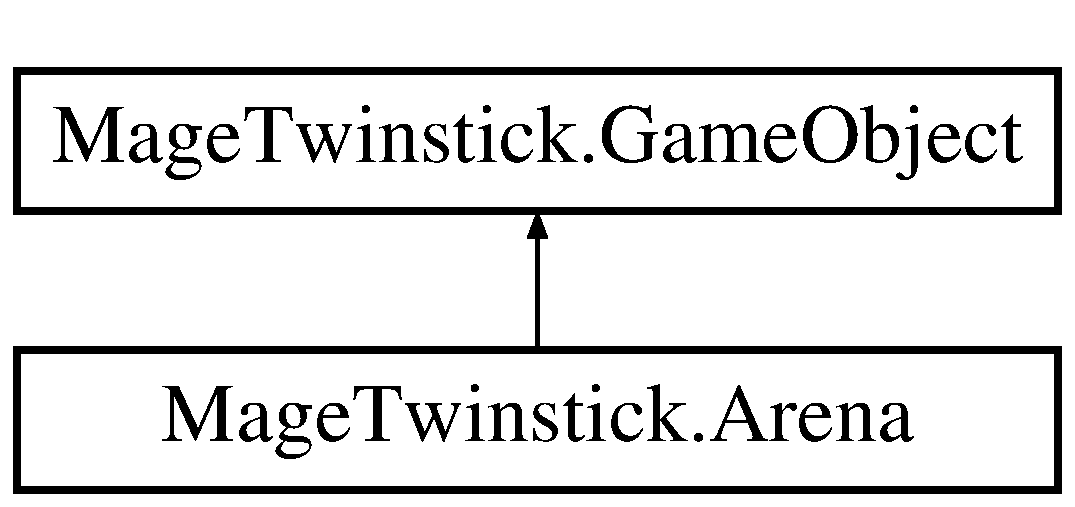
\includegraphics[height=2.000000cm]{class_mage_twinstick_1_1_arena}
\end{center}
\end{figure}
\subsection*{Public Member Functions}
\begin{DoxyCompactItemize}
\item 
\hypertarget{class_mage_twinstick_1_1_arena_aace14406dc02031e9739a08e5be7301b}{}{\bfseries Arena} (string image\+Path, \hyperlink{class_mage_twinstick_1_1_vector2_d}{Vector2\+D} start\+Pos, Rectangle \hyperlink{class_mage_twinstick_1_1_game_object_a5807df7f837dc87c8955a008d0b27b50}{display}, float \hyperlink{class_mage_twinstick_1_1_game_object_a5d21c31402c27c5a19f2a62d98720456}{animation\+Speed})\label{class_mage_twinstick_1_1_arena_aace14406dc02031e9739a08e5be7301b}

\item 
override void \hyperlink{class_mage_twinstick_1_1_arena_a12cdc5acc58ee006eb0b5a47507934fc}{On\+Collision} (\hyperlink{class_mage_twinstick_1_1_game_object}{Game\+Object} other)
\begin{DoxyCompactList}\small\item\em Abstract method for functionality when colliding with a specific \hyperlink{class_mage_twinstick_1_1_game_object}{Game\+Object} \end{DoxyCompactList}\end{DoxyCompactItemize}
\subsection*{Additional Inherited Members}


\subsection{Member Function Documentation}
\hypertarget{class_mage_twinstick_1_1_arena_a12cdc5acc58ee006eb0b5a47507934fc}{}\index{Mage\+Twinstick\+::\+Arena@{Mage\+Twinstick\+::\+Arena}!On\+Collision@{On\+Collision}}
\index{On\+Collision@{On\+Collision}!Mage\+Twinstick\+::\+Arena@{Mage\+Twinstick\+::\+Arena}}
\subsubsection[{On\+Collision(\+Game\+Object other)}]{\setlength{\rightskip}{0pt plus 5cm}override void Mage\+Twinstick.\+Arena.\+On\+Collision (
\begin{DoxyParamCaption}
\item[{{\bf Game\+Object}}]{other}
\end{DoxyParamCaption}
)\hspace{0.3cm}{\ttfamily [inline]}, {\ttfamily [virtual]}}\label{class_mage_twinstick_1_1_arena_a12cdc5acc58ee006eb0b5a47507934fc}


Abstract method for functionality when colliding with a specific \hyperlink{class_mage_twinstick_1_1_game_object}{Game\+Object} 


\begin{DoxyParams}{Parameters}
{\em other} & The other \hyperlink{class_mage_twinstick_1_1_game_object}{Game\+Object}\\
\hline
\end{DoxyParams}


Implements \hyperlink{class_mage_twinstick_1_1_game_object_a60f894a5ff911af7bfe3e4bd8abf253f}{Mage\+Twinstick.\+Game\+Object}.



The documentation for this class was generated from the following file\+:\begin{DoxyCompactItemize}
\item 
Arena.\+cs\end{DoxyCompactItemize}

\hypertarget{class_mage_twinstick_1_1_enemy_controller}{}\section{Mage\+Twinstick.\+Enemy\+Controller Class Reference}
\label{class_mage_twinstick_1_1_enemy_controller}\index{Mage\+Twinstick.\+Enemy\+Controller@{Mage\+Twinstick.\+Enemy\+Controller}}


The documentation for this class was generated from the following file\+:\begin{DoxyCompactItemize}
\item 
Enemy\+Controller.\+cs\end{DoxyCompactItemize}

\hypertarget{class_mage_twinstick_1_1_enemy_projectile}{}\section{Mage\+Twinstick.\+Enemy\+Projectile Class Reference}
\label{class_mage_twinstick_1_1_enemy_projectile}\index{Mage\+Twinstick.\+Enemy\+Projectile@{Mage\+Twinstick.\+Enemy\+Projectile}}
Inheritance diagram for Mage\+Twinstick.\+Enemy\+Projectile\+:\begin{figure}[H]
\begin{center}
\leavevmode
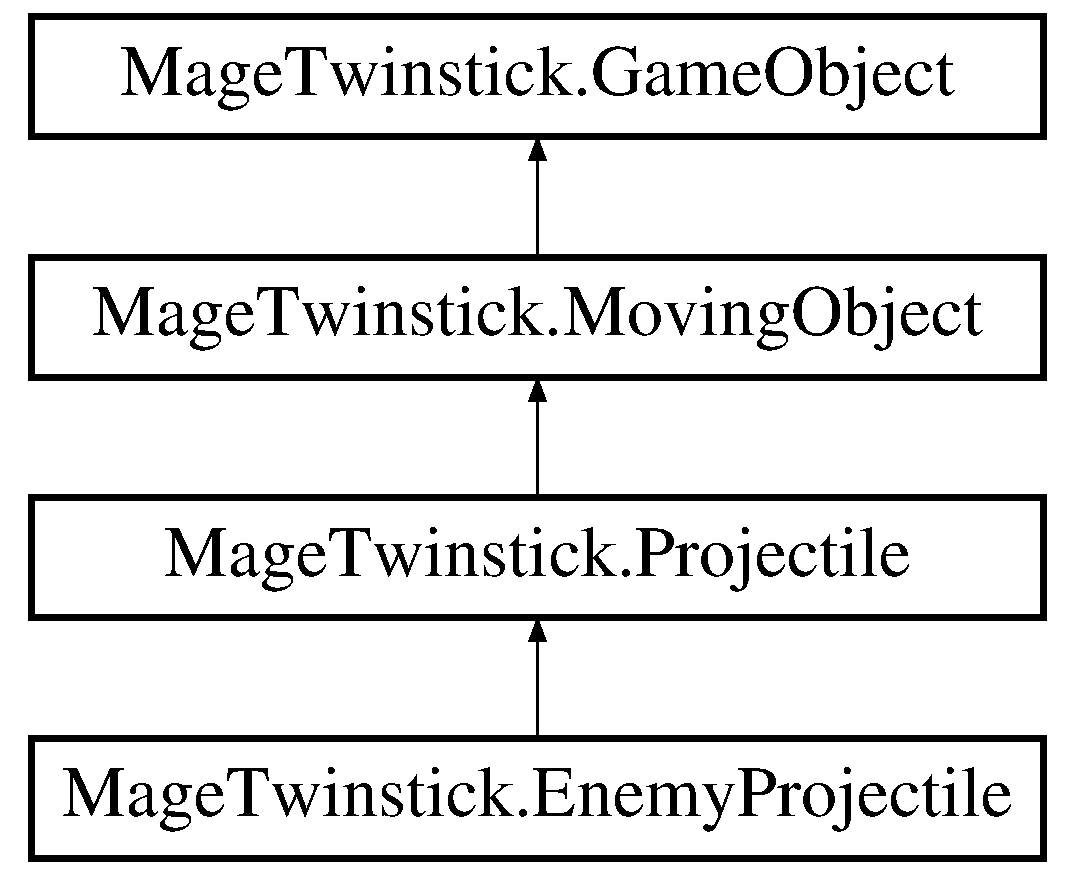
\includegraphics[height=4.000000cm]{class_mage_twinstick_1_1_enemy_projectile}
\end{center}
\end{figure}
\subsection*{Public Member Functions}
\begin{DoxyCompactItemize}
\item 
\hypertarget{class_mage_twinstick_1_1_enemy_projectile_aeddaa709304e1f22c45c82202b385352}{}{\bfseries Enemy\+Projectile} (float speed, string image\+Path, \hyperlink{class_mage_twinstick_1_1_vector2_d}{Vector2\+D} start\+Pos, Rectangle display, float animation\+Speed)\label{class_mage_twinstick_1_1_enemy_projectile_aeddaa709304e1f22c45c82202b385352}

\end{DoxyCompactItemize}
\subsection*{Additional Inherited Members}


The documentation for this class was generated from the following file\+:\begin{DoxyCompactItemize}
\item 
Enemy\+Projectile.\+cs\end{DoxyCompactItemize}

\hypertarget{class_mage_twinstick_1_1_enemy_spawner}{}\section{Mage\+Twinstick.\+Enemy\+Spawner Class Reference}
\label{class_mage_twinstick_1_1_enemy_spawner}\index{Mage\+Twinstick.\+Enemy\+Spawner@{Mage\+Twinstick.\+Enemy\+Spawner}}
\subsection*{Public Member Functions}
\begin{DoxyCompactItemize}
\item 
\hypertarget{class_mage_twinstick_1_1_enemy_spawner_abd353f77aec752709c47a110a15a1bb2}{}{\bfseries Enemy\+Spawner} (Rectangle display, \hyperlink{class_mage_twinstick_1_1_player}{Player} player)\label{class_mage_twinstick_1_1_enemy_spawner_abd353f77aec752709c47a110a15a1bb2}

\item 
virtual void \hyperlink{class_mage_twinstick_1_1_enemy_spawner_a4e22661d16cc2c9671eefe32fda8a42e}{Update} (float fps)
\end{DoxyCompactItemize}
\subsection*{Protected Attributes}
\begin{DoxyCompactItemize}
\item 
float \hyperlink{class_mage_twinstick_1_1_enemy_spawner_ae8e524a6c9480737390fcf8903c924b7}{angle}
\item 
float \hyperlink{class_mage_twinstick_1_1_enemy_spawner_afae9c62c10aab60fb5232880bdc58eef}{pos\+X}
\item 
float \hyperlink{class_mage_twinstick_1_1_enemy_spawner_a202528664dcf4d1107551469b7147a36}{pos\+Y}
\end{DoxyCompactItemize}


\subsection{Member Function Documentation}
\hypertarget{class_mage_twinstick_1_1_enemy_spawner_a4e22661d16cc2c9671eefe32fda8a42e}{}\index{Mage\+Twinstick\+::\+Enemy\+Spawner@{Mage\+Twinstick\+::\+Enemy\+Spawner}!Update@{Update}}
\index{Update@{Update}!Mage\+Twinstick\+::\+Enemy\+Spawner@{Mage\+Twinstick\+::\+Enemy\+Spawner}}
\subsubsection[{Update(float fps)}]{\setlength{\rightskip}{0pt plus 5cm}virtual void Mage\+Twinstick.\+Enemy\+Spawner.\+Update (
\begin{DoxyParamCaption}
\item[{float}]{fps}
\end{DoxyParamCaption}
)\hspace{0.3cm}{\ttfamily [inline]}, {\ttfamily [virtual]}}\label{class_mage_twinstick_1_1_enemy_spawner_a4e22661d16cc2c9671eefe32fda8a42e}
$<$Setting the enemy spawner to true, to make sure that only the appropriate number of enemies is spawned each round. 

\subsection{Member Data Documentation}
\hypertarget{class_mage_twinstick_1_1_enemy_spawner_ae8e524a6c9480737390fcf8903c924b7}{}\index{Mage\+Twinstick\+::\+Enemy\+Spawner@{Mage\+Twinstick\+::\+Enemy\+Spawner}!angle@{angle}}
\index{angle@{angle}!Mage\+Twinstick\+::\+Enemy\+Spawner@{Mage\+Twinstick\+::\+Enemy\+Spawner}}
\subsubsection[{angle}]{\setlength{\rightskip}{0pt plus 5cm}float Mage\+Twinstick.\+Enemy\+Spawner.\+angle\hspace{0.3cm}{\ttfamily [protected]}}\label{class_mage_twinstick_1_1_enemy_spawner_ae8e524a6c9480737390fcf8903c924b7}
Used to describe the angle in which the enemy will spawn \hypertarget{class_mage_twinstick_1_1_enemy_spawner_afae9c62c10aab60fb5232880bdc58eef}{}\index{Mage\+Twinstick\+::\+Enemy\+Spawner@{Mage\+Twinstick\+::\+Enemy\+Spawner}!pos\+X@{pos\+X}}
\index{pos\+X@{pos\+X}!Mage\+Twinstick\+::\+Enemy\+Spawner@{Mage\+Twinstick\+::\+Enemy\+Spawner}}
\subsubsection[{pos\+X}]{\setlength{\rightskip}{0pt plus 5cm}float Mage\+Twinstick.\+Enemy\+Spawner.\+pos\+X\hspace{0.3cm}{\ttfamily [protected]}}\label{class_mage_twinstick_1_1_enemy_spawner_afae9c62c10aab60fb5232880bdc58eef}
Used to calculate the position of the enemy on the X axis \hypertarget{class_mage_twinstick_1_1_enemy_spawner_a202528664dcf4d1107551469b7147a36}{}\index{Mage\+Twinstick\+::\+Enemy\+Spawner@{Mage\+Twinstick\+::\+Enemy\+Spawner}!pos\+Y@{pos\+Y}}
\index{pos\+Y@{pos\+Y}!Mage\+Twinstick\+::\+Enemy\+Spawner@{Mage\+Twinstick\+::\+Enemy\+Spawner}}
\subsubsection[{pos\+Y}]{\setlength{\rightskip}{0pt plus 5cm}float Mage\+Twinstick.\+Enemy\+Spawner.\+pos\+Y\hspace{0.3cm}{\ttfamily [protected]}}\label{class_mage_twinstick_1_1_enemy_spawner_a202528664dcf4d1107551469b7147a36}
Used to calculate the position of the enemy on the Y axis 

The documentation for this class was generated from the following file\+:\begin{DoxyCompactItemize}
\item 
Enemy\+Spawner.\+cs\end{DoxyCompactItemize}

\hypertarget{class_mage_twinstick_1_1_form1}{}\section{Mage\+Twinstick.\+Form1 Class Reference}
\label{class_mage_twinstick_1_1_form1}\index{Mage\+Twinstick.\+Form1@{Mage\+Twinstick.\+Form1}}
Inheritance diagram for Mage\+Twinstick.\+Form1\+:\begin{figure}[H]
\begin{center}
\leavevmode
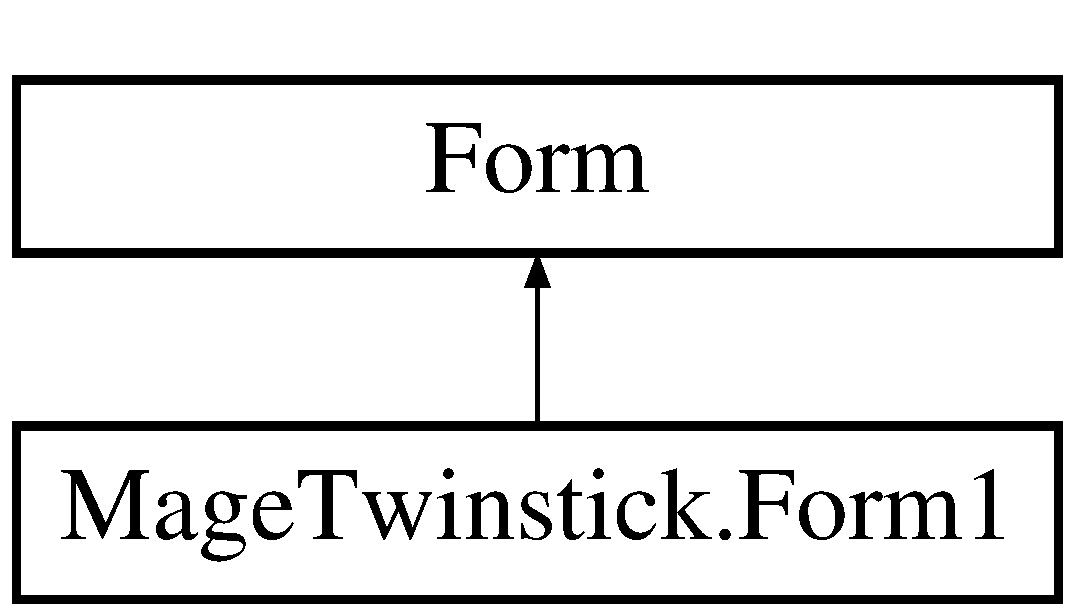
\includegraphics[height=2.000000cm]{class_mage_twinstick_1_1_form1}
\end{center}
\end{figure}
\subsection*{Protected Member Functions}
\begin{DoxyCompactItemize}
\item 
override void \hyperlink{class_mage_twinstick_1_1_form1_a0c6a13fd61a1b440f8c57c418238af9d}{Dispose} (bool disposing)
\begin{DoxyCompactList}\small\item\em Clean up any resources being used. \end{DoxyCompactList}\end{DoxyCompactItemize}


\subsection{Member Function Documentation}
\hypertarget{class_mage_twinstick_1_1_form1_a0c6a13fd61a1b440f8c57c418238af9d}{}\index{Mage\+Twinstick\+::\+Form1@{Mage\+Twinstick\+::\+Form1}!Dispose@{Dispose}}
\index{Dispose@{Dispose}!Mage\+Twinstick\+::\+Form1@{Mage\+Twinstick\+::\+Form1}}
\subsubsection[{Dispose(bool disposing)}]{\setlength{\rightskip}{0pt plus 5cm}override void Mage\+Twinstick.\+Form1.\+Dispose (
\begin{DoxyParamCaption}
\item[{bool}]{disposing}
\end{DoxyParamCaption}
)\hspace{0.3cm}{\ttfamily [inline]}, {\ttfamily [protected]}}\label{class_mage_twinstick_1_1_form1_a0c6a13fd61a1b440f8c57c418238af9d}


Clean up any resources being used. 


\begin{DoxyParams}{Parameters}
{\em disposing} & true if managed resources should be disposed; otherwise, false.\\
\hline
\end{DoxyParams}


The documentation for this class was generated from the following files\+:\begin{DoxyCompactItemize}
\item 
Form1.\+cs\item 
Form1.\+Designer.\+cs\end{DoxyCompactItemize}

\hypertarget{class_mage_twinstick_1_1_game_object}{}\section{Mage\+Twinstick.\+Game\+Object Class Reference}
\label{class_mage_twinstick_1_1_game_object}\index{Mage\+Twinstick.\+Game\+Object@{Mage\+Twinstick.\+Game\+Object}}


Superclass for anything that exsist in the Game\+World  


Inheritance diagram for Mage\+Twinstick.\+Game\+Object\+:\begin{figure}[H]
\begin{center}
\leavevmode
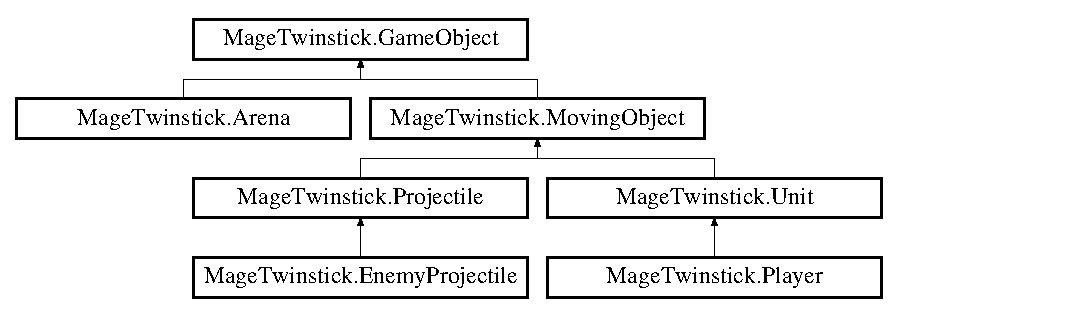
\includegraphics[height=4.000000cm]{class_mage_twinstick_1_1_game_object}
\end{center}
\end{figure}
\subsection*{Public Member Functions}
\begin{DoxyCompactItemize}
\item 
\hyperlink{class_mage_twinstick_1_1_game_object_a70fd6f506e37d368c4b5dc324286e0ec}{Game\+Object} (string image\+Path, \hyperlink{class_mage_twinstick_1_1_vector2_d}{Vector2\+D} start\+Pos, Rectangle \hyperlink{class_mage_twinstick_1_1_game_object_a5807df7f837dc87c8955a008d0b27b50}{display}, float \hyperlink{class_mage_twinstick_1_1_game_object_a5d21c31402c27c5a19f2a62d98720456}{animation\+Speed})
\begin{DoxyCompactList}\small\item\em \hyperlink{class_mage_twinstick_1_1_game_object}{Game\+Object} Constructor \end{DoxyCompactList}\item 
virtual void \hyperlink{class_mage_twinstick_1_1_game_object_a11628f4d9b508e2d976ca25f716b74f5}{Draw} (Graphics dc)
\begin{DoxyCompactList}\small\item\em draws the graphics in the Game\+World \end{DoxyCompactList}\item 
virtual void \hyperlink{class_mage_twinstick_1_1_game_object_a3de8248d06d234f8335525bbb28ccacc}{Update} (float fps)
\begin{DoxyCompactList}\small\item\em updates the information in the \hyperlink{class_mage_twinstick_1_1_game_object}{Game\+Object} \end{DoxyCompactList}\item 
virtual void \hyperlink{class_mage_twinstick_1_1_game_object_a35d6d9af3335b978c618ab73da1215a0}{Update\+Animation} (float fps)
\begin{DoxyCompactList}\small\item\em Animates the sprite on the \hyperlink{class_mage_twinstick_1_1_game_object}{Game\+Object} \end{DoxyCompactList}\item 
void \hyperlink{class_mage_twinstick_1_1_game_object_a5ed64726e236792a162c2899b7446d66}{Check\+Collision} ()
\begin{DoxyCompactList}\small\item\em Checks for collision with other Game\+Objects \end{DoxyCompactList}\item 
bool \hyperlink{class_mage_twinstick_1_1_game_object_a024097f67b0a8b2f38451e8df05b6b1d}{Is\+Colliding\+With} (\hyperlink{class_mage_twinstick_1_1_game_object}{Game\+Object} other)
\begin{DoxyCompactList}\small\item\em Checks for collision with a specific \hyperlink{class_mage_twinstick_1_1_game_object}{Game\+Object} \end{DoxyCompactList}\item 
abstract void \hyperlink{class_mage_twinstick_1_1_game_object_a60f894a5ff911af7bfe3e4bd8abf253f}{On\+Collision} (\hyperlink{class_mage_twinstick_1_1_game_object}{Game\+Object} other)
\begin{DoxyCompactList}\small\item\em Abstract method for functionality when colliding with a specific \hyperlink{class_mage_twinstick_1_1_game_object}{Game\+Object} \end{DoxyCompactList}\end{DoxyCompactItemize}
\subsection*{Protected Attributes}
\begin{DoxyCompactItemize}
\item 
\hypertarget{class_mage_twinstick_1_1_game_object_a0d553d62b8d1e865b6f106c6b3b110fe}{}Image \hyperlink{class_mage_twinstick_1_1_game_object_a0d553d62b8d1e865b6f106c6b3b110fe}{sprite}\label{class_mage_twinstick_1_1_game_object_a0d553d62b8d1e865b6f106c6b3b110fe}

\begin{DoxyCompactList}\small\item\em Image sprite for the \hyperlink{class_mage_twinstick_1_1_game_object}{Game\+Object}. \end{DoxyCompactList}\item 
\hypertarget{class_mage_twinstick_1_1_game_object_a5807df7f837dc87c8955a008d0b27b50}{}Rectangle \hyperlink{class_mage_twinstick_1_1_game_object_a5807df7f837dc87c8955a008d0b27b50}{display}\label{class_mage_twinstick_1_1_game_object_a5807df7f837dc87c8955a008d0b27b50}

\begin{DoxyCompactList}\small\item\em Rectangle for the display. \end{DoxyCompactList}\item 
\hypertarget{class_mage_twinstick_1_1_game_object_a8cc6f0911171f56d011803b3ab70a7b5}{}List$<$ Image $>$ \hyperlink{class_mage_twinstick_1_1_game_object_a8cc6f0911171f56d011803b3ab70a7b5}{animation\+Frames}\label{class_mage_twinstick_1_1_game_object_a8cc6f0911171f56d011803b3ab70a7b5}

\begin{DoxyCompactList}\small\item\em List of images for animated objects. \end{DoxyCompactList}\item 
\hypertarget{class_mage_twinstick_1_1_game_object_a5a94b322db89e1230005a33f1205e742}{}float \hyperlink{class_mage_twinstick_1_1_game_object_a5a94b322db89e1230005a33f1205e742}{current\+Frame\+Index}\label{class_mage_twinstick_1_1_game_object_a5a94b322db89e1230005a33f1205e742}

\begin{DoxyCompactList}\small\item\em the current Frame in the animation \end{DoxyCompactList}\item 
\hypertarget{class_mage_twinstick_1_1_game_object_a5d21c31402c27c5a19f2a62d98720456}{}float \hyperlink{class_mage_twinstick_1_1_game_object_a5d21c31402c27c5a19f2a62d98720456}{animation\+Speed}\label{class_mage_twinstick_1_1_game_object_a5d21c31402c27c5a19f2a62d98720456}

\begin{DoxyCompactList}\small\item\em the speed of the animation \end{DoxyCompactList}\end{DoxyCompactItemize}
\subsection*{Properties}
\begin{DoxyCompactItemize}
\item 
\hyperlink{class_mage_twinstick_1_1_vector2_d}{Vector2\+D} \hyperlink{class_mage_twinstick_1_1_game_object_a74cf54e9808f3a9f93fa5c837076a7f0}{Position}\hspace{0.3cm}{\ttfamily  \mbox{[}get, set\mbox{]}}
\begin{DoxyCompactList}\small\item\em 2\+D Vector for the \hyperlink{class_mage_twinstick_1_1_game_object}{Game\+Object} position \end{DoxyCompactList}\item 
Rectangle\+F \hyperlink{class_mage_twinstick_1_1_game_object_a66a2645b4fda01d5dd2f5e311c338b90}{Collision\+Box}\hspace{0.3cm}{\ttfamily  \mbox{[}get\mbox{]}}
\begin{DoxyCompactList}\small\item\em Rectanglge for the Game\+Objects collider \end{DoxyCompactList}\end{DoxyCompactItemize}


\subsection{Detailed Description}
Superclass for anything that exsist in the Game\+World 



\subsection{Constructor \& Destructor Documentation}
\hypertarget{class_mage_twinstick_1_1_game_object_a70fd6f506e37d368c4b5dc324286e0ec}{}\index{Mage\+Twinstick\+::\+Game\+Object@{Mage\+Twinstick\+::\+Game\+Object}!Game\+Object@{Game\+Object}}
\index{Game\+Object@{Game\+Object}!Mage\+Twinstick\+::\+Game\+Object@{Mage\+Twinstick\+::\+Game\+Object}}
\subsubsection[{Game\+Object(string image\+Path, Vector2\+D start\+Pos, Rectangle display, float animation\+Speed)}]{\setlength{\rightskip}{0pt plus 5cm}Mage\+Twinstick.\+Game\+Object.\+Game\+Object (
\begin{DoxyParamCaption}
\item[{string}]{image\+Path, }
\item[{{\bf Vector2\+D}}]{start\+Pos, }
\item[{Rectangle}]{display, }
\item[{float}]{animation\+Speed}
\end{DoxyParamCaption}
)\hspace{0.3cm}{\ttfamily [inline]}}\label{class_mage_twinstick_1_1_game_object_a70fd6f506e37d368c4b5dc324286e0ec}


\hyperlink{class_mage_twinstick_1_1_game_object}{Game\+Object} Constructor 


\begin{DoxyParams}{Parameters}
{\em image\+Path} & Image path for the sprite\\
\hline
{\em start\+Pos} & The starting position of the \hyperlink{class_mage_twinstick_1_1_game_object}{Game\+Object}\\
\hline
{\em display} & Rectangle for the diplay\\
\hline
{\em animation\+Speed} & Animation speed for animated objects\\
\hline
\end{DoxyParams}


\subsection{Member Function Documentation}
\hypertarget{class_mage_twinstick_1_1_game_object_a5ed64726e236792a162c2899b7446d66}{}\index{Mage\+Twinstick\+::\+Game\+Object@{Mage\+Twinstick\+::\+Game\+Object}!Check\+Collision@{Check\+Collision}}
\index{Check\+Collision@{Check\+Collision}!Mage\+Twinstick\+::\+Game\+Object@{Mage\+Twinstick\+::\+Game\+Object}}
\subsubsection[{Check\+Collision()}]{\setlength{\rightskip}{0pt plus 5cm}void Mage\+Twinstick.\+Game\+Object.\+Check\+Collision (
\begin{DoxyParamCaption}
{}
\end{DoxyParamCaption}
)\hspace{0.3cm}{\ttfamily [inline]}}\label{class_mage_twinstick_1_1_game_object_a5ed64726e236792a162c2899b7446d66}


Checks for collision with other Game\+Objects 

\hypertarget{class_mage_twinstick_1_1_game_object_a11628f4d9b508e2d976ca25f716b74f5}{}\index{Mage\+Twinstick\+::\+Game\+Object@{Mage\+Twinstick\+::\+Game\+Object}!Draw@{Draw}}
\index{Draw@{Draw}!Mage\+Twinstick\+::\+Game\+Object@{Mage\+Twinstick\+::\+Game\+Object}}
\subsubsection[{Draw(\+Graphics dc)}]{\setlength{\rightskip}{0pt plus 5cm}virtual void Mage\+Twinstick.\+Game\+Object.\+Draw (
\begin{DoxyParamCaption}
\item[{Graphics}]{dc}
\end{DoxyParamCaption}
)\hspace{0.3cm}{\ttfamily [inline]}, {\ttfamily [virtual]}}\label{class_mage_twinstick_1_1_game_object_a11628f4d9b508e2d976ca25f716b74f5}


draws the graphics in the Game\+World 


\begin{DoxyParams}{Parameters}
{\em dc} & G\+D\+I+ class for drawing the sprite\\
\hline
\end{DoxyParams}


Reimplemented in \hyperlink{class_mage_twinstick_1_1_player_a2ccf76e50c0e5fa6642da04a4a5c4fa8}{Mage\+Twinstick.\+Player}.

\hypertarget{class_mage_twinstick_1_1_game_object_a024097f67b0a8b2f38451e8df05b6b1d}{}\index{Mage\+Twinstick\+::\+Game\+Object@{Mage\+Twinstick\+::\+Game\+Object}!Is\+Colliding\+With@{Is\+Colliding\+With}}
\index{Is\+Colliding\+With@{Is\+Colliding\+With}!Mage\+Twinstick\+::\+Game\+Object@{Mage\+Twinstick\+::\+Game\+Object}}
\subsubsection[{Is\+Colliding\+With(\+Game\+Object other)}]{\setlength{\rightskip}{0pt plus 5cm}bool Mage\+Twinstick.\+Game\+Object.\+Is\+Colliding\+With (
\begin{DoxyParamCaption}
\item[{{\bf Game\+Object}}]{other}
\end{DoxyParamCaption}
)\hspace{0.3cm}{\ttfamily [inline]}}\label{class_mage_twinstick_1_1_game_object_a024097f67b0a8b2f38451e8df05b6b1d}


Checks for collision with a specific \hyperlink{class_mage_twinstick_1_1_game_object}{Game\+Object} 


\begin{DoxyParams}{Parameters}
{\em other} & The other \hyperlink{class_mage_twinstick_1_1_game_object}{Game\+Object}\\
\hline
\end{DoxyParams}
\begin{DoxyReturn}{Returns}

\end{DoxyReturn}
\hypertarget{class_mage_twinstick_1_1_game_object_a60f894a5ff911af7bfe3e4bd8abf253f}{}\index{Mage\+Twinstick\+::\+Game\+Object@{Mage\+Twinstick\+::\+Game\+Object}!On\+Collision@{On\+Collision}}
\index{On\+Collision@{On\+Collision}!Mage\+Twinstick\+::\+Game\+Object@{Mage\+Twinstick\+::\+Game\+Object}}
\subsubsection[{On\+Collision(\+Game\+Object other)}]{\setlength{\rightskip}{0pt plus 5cm}abstract void Mage\+Twinstick.\+Game\+Object.\+On\+Collision (
\begin{DoxyParamCaption}
\item[{{\bf Game\+Object}}]{other}
\end{DoxyParamCaption}
)\hspace{0.3cm}{\ttfamily [pure virtual]}}\label{class_mage_twinstick_1_1_game_object_a60f894a5ff911af7bfe3e4bd8abf253f}


Abstract method for functionality when colliding with a specific \hyperlink{class_mage_twinstick_1_1_game_object}{Game\+Object} 


\begin{DoxyParams}{Parameters}
{\em other} & The other \hyperlink{class_mage_twinstick_1_1_game_object}{Game\+Object}\\
\hline
\end{DoxyParams}


Implemented in \hyperlink{class_mage_twinstick_1_1_player_adb9172ee6c160eb686076749d29be061}{Mage\+Twinstick.\+Player}, \hyperlink{class_mage_twinstick_1_1_projectile_ad646d013997eceb12a0ac2f5df56d3bb}{Mage\+Twinstick.\+Projectile}, and \hyperlink{class_mage_twinstick_1_1_arena_a12cdc5acc58ee006eb0b5a47507934fc}{Mage\+Twinstick.\+Arena}.

\hypertarget{class_mage_twinstick_1_1_game_object_a3de8248d06d234f8335525bbb28ccacc}{}\index{Mage\+Twinstick\+::\+Game\+Object@{Mage\+Twinstick\+::\+Game\+Object}!Update@{Update}}
\index{Update@{Update}!Mage\+Twinstick\+::\+Game\+Object@{Mage\+Twinstick\+::\+Game\+Object}}
\subsubsection[{Update(float fps)}]{\setlength{\rightskip}{0pt plus 5cm}virtual void Mage\+Twinstick.\+Game\+Object.\+Update (
\begin{DoxyParamCaption}
\item[{float}]{fps}
\end{DoxyParamCaption}
)\hspace{0.3cm}{\ttfamily [inline]}, {\ttfamily [virtual]}}\label{class_mage_twinstick_1_1_game_object_a3de8248d06d234f8335525bbb28ccacc}


updates the information in the \hyperlink{class_mage_twinstick_1_1_game_object}{Game\+Object} 


\begin{DoxyParams}{Parameters}
{\em fps} & Fps used to update based on time\\
\hline
\end{DoxyParams}


Reimplemented in \hyperlink{class_mage_twinstick_1_1_player_a5324e0350784da0f66369ec5ef52516a}{Mage\+Twinstick.\+Player}, and \hyperlink{class_mage_twinstick_1_1_projectile_a9208eff25bc92289191d5470bbc7015a}{Mage\+Twinstick.\+Projectile}.

\hypertarget{class_mage_twinstick_1_1_game_object_a35d6d9af3335b978c618ab73da1215a0}{}\index{Mage\+Twinstick\+::\+Game\+Object@{Mage\+Twinstick\+::\+Game\+Object}!Update\+Animation@{Update\+Animation}}
\index{Update\+Animation@{Update\+Animation}!Mage\+Twinstick\+::\+Game\+Object@{Mage\+Twinstick\+::\+Game\+Object}}
\subsubsection[{Update\+Animation(float fps)}]{\setlength{\rightskip}{0pt plus 5cm}virtual void Mage\+Twinstick.\+Game\+Object.\+Update\+Animation (
\begin{DoxyParamCaption}
\item[{float}]{fps}
\end{DoxyParamCaption}
)\hspace{0.3cm}{\ttfamily [inline]}, {\ttfamily [virtual]}}\label{class_mage_twinstick_1_1_game_object_a35d6d9af3335b978c618ab73da1215a0}


Animates the sprite on the \hyperlink{class_mage_twinstick_1_1_game_object}{Game\+Object} 


\begin{DoxyParams}{Parameters}
{\em fps} & Fps used to update based on time\\
\hline
\end{DoxyParams}


\subsection{Property Documentation}
\hypertarget{class_mage_twinstick_1_1_game_object_a66a2645b4fda01d5dd2f5e311c338b90}{}\index{Mage\+Twinstick\+::\+Game\+Object@{Mage\+Twinstick\+::\+Game\+Object}!Collision\+Box@{Collision\+Box}}
\index{Collision\+Box@{Collision\+Box}!Mage\+Twinstick\+::\+Game\+Object@{Mage\+Twinstick\+::\+Game\+Object}}
\subsubsection[{Collision\+Box}]{\setlength{\rightskip}{0pt plus 5cm}Rectangle\+F Mage\+Twinstick.\+Game\+Object.\+Collision\+Box\hspace{0.3cm}{\ttfamily [get]}}\label{class_mage_twinstick_1_1_game_object_a66a2645b4fda01d5dd2f5e311c338b90}


Rectanglge for the Game\+Objects collider 

\hypertarget{class_mage_twinstick_1_1_game_object_a74cf54e9808f3a9f93fa5c837076a7f0}{}\index{Mage\+Twinstick\+::\+Game\+Object@{Mage\+Twinstick\+::\+Game\+Object}!Position@{Position}}
\index{Position@{Position}!Mage\+Twinstick\+::\+Game\+Object@{Mage\+Twinstick\+::\+Game\+Object}}
\subsubsection[{Position}]{\setlength{\rightskip}{0pt plus 5cm}{\bf Vector2\+D} Mage\+Twinstick.\+Game\+Object.\+Position\hspace{0.3cm}{\ttfamily [get]}, {\ttfamily [set]}}\label{class_mage_twinstick_1_1_game_object_a74cf54e9808f3a9f93fa5c837076a7f0}


2\+D Vector for the \hyperlink{class_mage_twinstick_1_1_game_object}{Game\+Object} position 



The documentation for this class was generated from the following file\+:\begin{DoxyCompactItemize}
\item 
Game\+Object.\+cs\end{DoxyCompactItemize}

\hypertarget{class_mage_twinstick_1_1_game_world}{}\section{Mage\+Twinstick.\+Game\+World Class Reference}
\label{class_mage_twinstick_1_1_game_world}\index{Mage\+Twinstick.\+Game\+World@{Mage\+Twinstick.\+Game\+World}}
\subsection*{Public Member Functions}
\begin{DoxyCompactItemize}
\item 
\hypertarget{class_mage_twinstick_1_1_game_world_a270f04b1de26513f7893e361303fb129}{}{\bfseries Game\+World} (Graphics dc, Rectangle display)\label{class_mage_twinstick_1_1_game_world_a270f04b1de26513f7893e361303fb129}

\item 
\hypertarget{class_mage_twinstick_1_1_game_world_adb5bdbb96b081dfc7e2ed7a9b2acfa10}{}void {\bfseries Setup\+World} ()\label{class_mage_twinstick_1_1_game_world_adb5bdbb96b081dfc7e2ed7a9b2acfa10}

\item 
\hypertarget{class_mage_twinstick_1_1_game_world_a7a03f6b9f40b1e3e9aed96a614caf5e3}{}void {\bfseries Game\+Loop} ()\label{class_mage_twinstick_1_1_game_world_a7a03f6b9f40b1e3e9aed96a614caf5e3}

\item 
\hypertarget{class_mage_twinstick_1_1_game_world_aad92b4d3c95491f04ac4885d96c15c3c}{}void {\bfseries Draw} ()\label{class_mage_twinstick_1_1_game_world_aad92b4d3c95491f04ac4885d96c15c3c}

\item 
\hypertarget{class_mage_twinstick_1_1_game_world_a3912f8f9ec0acd789eb46e1abcfcf2de}{}void {\bfseries Update} ()\label{class_mage_twinstick_1_1_game_world_a3912f8f9ec0acd789eb46e1abcfcf2de}

\item 
\hypertarget{class_mage_twinstick_1_1_game_world_a6b30c5cbcee01e32068f0d2f117f96fb}{}void {\bfseries Update\+Animation} ()\label{class_mage_twinstick_1_1_game_world_a6b30c5cbcee01e32068f0d2f117f96fb}

\end{DoxyCompactItemize}
\subsection*{Properties}
\begin{DoxyCompactItemize}
\item 
\hypertarget{class_mage_twinstick_1_1_game_world_aa08512629d71365bea26ea059020f4ca}{}static List$<$ \hyperlink{class_mage_twinstick_1_1_game_object}{Game\+Object} $>$ {\bfseries Objects}\hspace{0.3cm}{\ttfamily  \mbox{[}get, set\mbox{]}}\label{class_mage_twinstick_1_1_game_world_aa08512629d71365bea26ea059020f4ca}

\item 
\hypertarget{class_mage_twinstick_1_1_game_world_af930b76068ef6637bb77fdcfd877a8f1}{}static List$<$ \hyperlink{class_mage_twinstick_1_1_game_object}{Game\+Object} $>$ {\bfseries Objects\+To\+Remove} = new List$<$\hyperlink{class_mage_twinstick_1_1_game_object}{Game\+Object}$>$()\hspace{0.3cm}{\ttfamily  \mbox{[}get, set\mbox{]}}\label{class_mage_twinstick_1_1_game_world_af930b76068ef6637bb77fdcfd877a8f1}

\item 
\hypertarget{class_mage_twinstick_1_1_game_world_a70ecede9da55d25220e0f524f760bcff}{}static List$<$ \hyperlink{class_mage_twinstick_1_1_game_object}{Game\+Object} $>$ {\bfseries Objects\+To\+Add} = new List$<$\hyperlink{class_mage_twinstick_1_1_game_object}{Game\+Object}$>$()\hspace{0.3cm}{\ttfamily  \mbox{[}get, set\mbox{]}}\label{class_mage_twinstick_1_1_game_world_a70ecede9da55d25220e0f524f760bcff}

\end{DoxyCompactItemize}


The documentation for this class was generated from the following file\+:\begin{DoxyCompactItemize}
\item 
Game\+World.\+cs\end{DoxyCompactItemize}

\hypertarget{class_mage_twinstick_1_1_melee_enemy}{}\section{Mage\+Twinstick.\+Melee\+Enemy Class Reference}
\label{class_mage_twinstick_1_1_melee_enemy}\index{Mage\+Twinstick.\+Melee\+Enemy@{Mage\+Twinstick.\+Melee\+Enemy}}


Inherits Mage\+Twinstick.\+Enemy.

\subsection*{Public Member Functions}
\begin{DoxyCompactItemize}
\item 
\hypertarget{class_mage_twinstick_1_1_melee_enemy_a57032b177c12225e99ce837002bead9b}{}{\bfseries Melee\+Enemy} (float speed, int health, string image\+Path, \hyperlink{class_mage_twinstick_1_1_vector2_d}{Vector2\+D} start\+Pos, Rectangle display, float animation\+Speed)\label{class_mage_twinstick_1_1_melee_enemy_a57032b177c12225e99ce837002bead9b}

\end{DoxyCompactItemize}


The documentation for this class was generated from the following file\+:\begin{DoxyCompactItemize}
\item 
Melee\+Enemy.\+cs\end{DoxyCompactItemize}

\hypertarget{class_mage_twinstick_1_1_moving_object}{}\section{Mage\+Twinstick.\+Moving\+Object Class Reference}
\label{class_mage_twinstick_1_1_moving_object}\index{Mage\+Twinstick.\+Moving\+Object@{Mage\+Twinstick.\+Moving\+Object}}


superclass for any object that moves  


Inheritance diagram for Mage\+Twinstick.\+Moving\+Object\+:\begin{figure}[H]
\begin{center}
\leavevmode
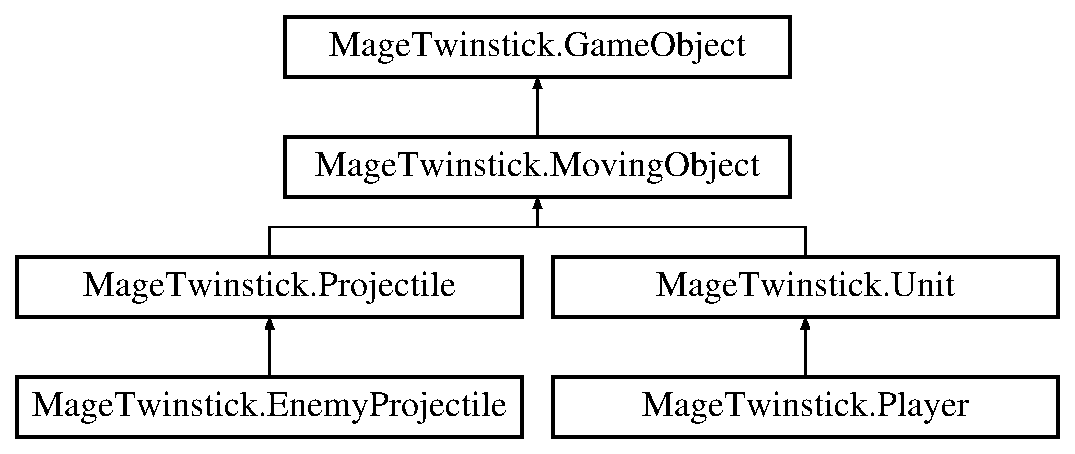
\includegraphics[height=4.000000cm]{class_mage_twinstick_1_1_moving_object}
\end{center}
\end{figure}
\subsection*{Public Member Functions}
\begin{DoxyCompactItemize}
\item 
\hyperlink{class_mage_twinstick_1_1_moving_object_ab600a7d67a921669d7021f9c8b7b9891}{Moving\+Object} (float speed, string image\+Path, \hyperlink{class_mage_twinstick_1_1_vector2_d}{Vector2\+D} start\+Pos, Rectangle \hyperlink{class_mage_twinstick_1_1_game_object_a5807df7f837dc87c8955a008d0b27b50}{display}, float \hyperlink{class_mage_twinstick_1_1_game_object_a5d21c31402c27c5a19f2a62d98720456}{animation\+Speed})
\begin{DoxyCompactList}\small\item\em constructer for movingobject \end{DoxyCompactList}\end{DoxyCompactItemize}
\subsection*{Protected Attributes}
\begin{DoxyCompactItemize}
\item 
\hypertarget{class_mage_twinstick_1_1_moving_object_ac7f09bc1fd21342a3c68b1d25c7e209d}{}float {\bfseries speed}\label{class_mage_twinstick_1_1_moving_object_ac7f09bc1fd21342a3c68b1d25c7e209d}

\item 
\hypertarget{class_mage_twinstick_1_1_moving_object_a93fbd4b287c423a80a525f4e45b93279}{}double {\bfseries angle}\label{class_mage_twinstick_1_1_moving_object_a93fbd4b287c423a80a525f4e45b93279}

\end{DoxyCompactItemize}
\subsection*{Additional Inherited Members}


\subsection{Detailed Description}
superclass for any object that moves 



\subsection{Constructor \& Destructor Documentation}
\hypertarget{class_mage_twinstick_1_1_moving_object_ab600a7d67a921669d7021f9c8b7b9891}{}\index{Mage\+Twinstick\+::\+Moving\+Object@{Mage\+Twinstick\+::\+Moving\+Object}!Moving\+Object@{Moving\+Object}}
\index{Moving\+Object@{Moving\+Object}!Mage\+Twinstick\+::\+Moving\+Object@{Mage\+Twinstick\+::\+Moving\+Object}}
\subsubsection[{Moving\+Object(float speed, string image\+Path, Vector2\+D start\+Pos, Rectangle display, float animation\+Speed)}]{\setlength{\rightskip}{0pt plus 5cm}Mage\+Twinstick.\+Moving\+Object.\+Moving\+Object (
\begin{DoxyParamCaption}
\item[{float}]{speed, }
\item[{string}]{image\+Path, }
\item[{{\bf Vector2\+D}}]{start\+Pos, }
\item[{Rectangle}]{display, }
\item[{float}]{animation\+Speed}
\end{DoxyParamCaption}
)\hspace{0.3cm}{\ttfamily [inline]}}\label{class_mage_twinstick_1_1_moving_object_ab600a7d67a921669d7021f9c8b7b9891}


constructer for movingobject 


\begin{DoxyParams}{Parameters}
{\em speed} & the movementspeed of the object\\
\hline
{\em image\+Path} & Path to the sprite\\
\hline
{\em start\+Pos} & Position to place the sprite\\
\hline
{\em display} & The displayrectangle\\
\hline
{\em animation\+Speed} & animatinospeed\\
\hline
\end{DoxyParams}


The documentation for this class was generated from the following file\+:\begin{DoxyCompactItemize}
\item 
Moving\+Object.\+cs\end{DoxyCompactItemize}

\hypertarget{class_mage_twinstick_1_1_player}{}\section{Mage\+Twinstick.\+Player Class Reference}
\label{class_mage_twinstick_1_1_player}\index{Mage\+Twinstick.\+Player@{Mage\+Twinstick.\+Player}}


the unit the player controls  


Inheritance diagram for Mage\+Twinstick.\+Player\+:\begin{figure}[H]
\begin{center}
\leavevmode
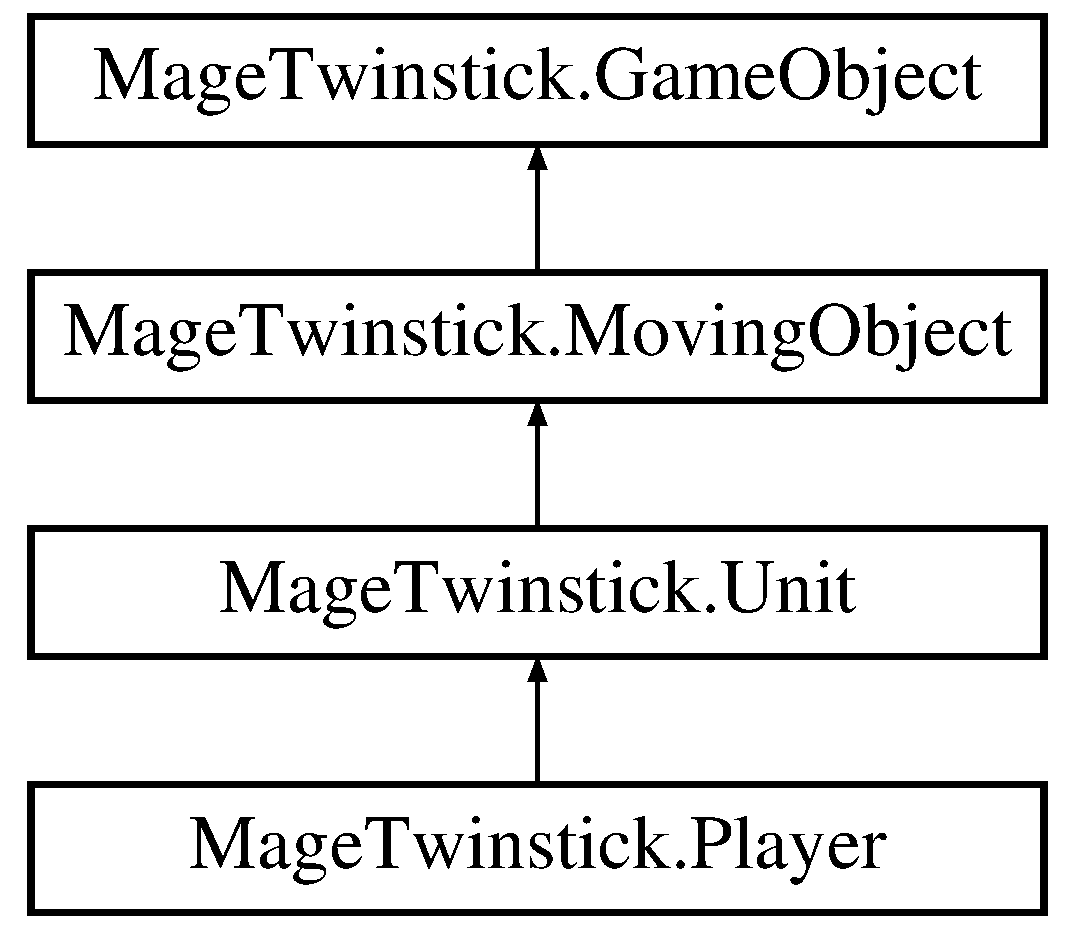
\includegraphics[height=4.000000cm]{class_mage_twinstick_1_1_player}
\end{center}
\end{figure}
\subsection*{Public Member Functions}
\begin{DoxyCompactItemize}
\item 
\hyperlink{class_mage_twinstick_1_1_player_ab0f3c00d033f0f20e743c04ae0eb6b11}{Player} (float speed, int health, string image\+Path, \hyperlink{class_mage_twinstick_1_1_vector2_d}{Vector2\+D} start\+Pos, Rectangle \hyperlink{class_mage_twinstick_1_1_game_object_a5807df7f837dc87c8955a008d0b27b50}{display}, float \hyperlink{class_mage_twinstick_1_1_game_object_a5d21c31402c27c5a19f2a62d98720456}{animation\+Speed})
\begin{DoxyCompactList}\small\item\em \hyperlink{class_mage_twinstick_1_1_player}{Player} constructor \end{DoxyCompactList}\item 
override void \hyperlink{class_mage_twinstick_1_1_player_a5324e0350784da0f66369ec5ef52516a}{Update} (float fps)
\begin{DoxyCompactList}\small\item\em move the character in the direction of the keys \end{DoxyCompactList}\item 
override void \hyperlink{class_mage_twinstick_1_1_player_adb9172ee6c160eb686076749d29be061}{On\+Collision} (\hyperlink{class_mage_twinstick_1_1_game_object}{Game\+Object} other)
\begin{DoxyCompactList}\small\item\em Detects Collision with other \hyperlink{class_mage_twinstick_1_1_game_object}{Game\+Object} objects \end{DoxyCompactList}\item 
override void \hyperlink{class_mage_twinstick_1_1_player_a2ccf76e50c0e5fa6642da04a4a5c4fa8}{Draw} (Graphics dc)
\begin{DoxyCompactList}\small\item\em draws the Graphics in the Game\+World \end{DoxyCompactList}\item 
override void \hyperlink{class_mage_twinstick_1_1_player_a418c80bddb416cd2cdd180ab21831f57}{Attack} ()
\begin{DoxyCompactList}\small\item\em attacks by adding a Projetcile in front of the player \end{DoxyCompactList}\end{DoxyCompactItemize}
\subsection*{Properties}
\begin{DoxyCompactItemize}
\item 
float \hyperlink{class_mage_twinstick_1_1_player_a0c30b0fbc931346ba557a49ea8e26b1d}{Mana}\hspace{0.3cm}{\ttfamily  \mbox{[}get, set\mbox{]}}
\begin{DoxyCompactList}\small\item\em Auto property for mana \end{DoxyCompactList}\item 
float \hyperlink{class_mage_twinstick_1_1_player_aa4b4878249b47797666fb77c82184533}{Score}\hspace{0.3cm}{\ttfamily  \mbox{[}get, set\mbox{]}}
\begin{DoxyCompactList}\small\item\em Auto property for score \end{DoxyCompactList}\end{DoxyCompactItemize}
\subsection*{Additional Inherited Members}


\subsection{Detailed Description}
the unit the player controls 



\subsection{Constructor \& Destructor Documentation}
\hypertarget{class_mage_twinstick_1_1_player_ab0f3c00d033f0f20e743c04ae0eb6b11}{}\index{Mage\+Twinstick\+::\+Player@{Mage\+Twinstick\+::\+Player}!Player@{Player}}
\index{Player@{Player}!Mage\+Twinstick\+::\+Player@{Mage\+Twinstick\+::\+Player}}
\subsubsection[{Player(float speed, int health, string image\+Path, Vector2\+D start\+Pos, Rectangle display, float animation\+Speed)}]{\setlength{\rightskip}{0pt plus 5cm}Mage\+Twinstick.\+Player.\+Player (
\begin{DoxyParamCaption}
\item[{float}]{speed, }
\item[{int}]{health, }
\item[{string}]{image\+Path, }
\item[{{\bf Vector2\+D}}]{start\+Pos, }
\item[{Rectangle}]{display, }
\item[{float}]{animation\+Speed}
\end{DoxyParamCaption}
)\hspace{0.3cm}{\ttfamily [inline]}}\label{class_mage_twinstick_1_1_player_ab0f3c00d033f0f20e743c04ae0eb6b11}


\hyperlink{class_mage_twinstick_1_1_player}{Player} constructor 


\begin{DoxyParams}{Parameters}
{\em speed} & The \hyperlink{class_mage_twinstick_1_1_player}{Player} movement speed\\
\hline
{\em health} & The \hyperlink{class_mage_twinstick_1_1_player}{Player} health\\
\hline
{\em image\+Path} & The path to the \hyperlink{class_mage_twinstick_1_1_player}{Player} sprite\\
\hline
{\em start\+Pos} & The \hyperlink{class_mage_twinstick_1_1_player}{Player} starting position\\
\hline
{\em display} & The display rectangle\\
\hline
{\em animation\+Speed} & The animation speed for the \hyperlink{class_mage_twinstick_1_1_player}{Player}\\
\hline
\end{DoxyParams}


\subsection{Member Function Documentation}
\hypertarget{class_mage_twinstick_1_1_player_a418c80bddb416cd2cdd180ab21831f57}{}\index{Mage\+Twinstick\+::\+Player@{Mage\+Twinstick\+::\+Player}!Attack@{Attack}}
\index{Attack@{Attack}!Mage\+Twinstick\+::\+Player@{Mage\+Twinstick\+::\+Player}}
\subsubsection[{Attack()}]{\setlength{\rightskip}{0pt plus 5cm}override void Mage\+Twinstick.\+Player.\+Attack (
\begin{DoxyParamCaption}
{}
\end{DoxyParamCaption}
)\hspace{0.3cm}{\ttfamily [inline]}, {\ttfamily [virtual]}}\label{class_mage_twinstick_1_1_player_a418c80bddb416cd2cdd180ab21831f57}


attacks by adding a Projetcile in front of the player 



Implements \hyperlink{class_mage_twinstick_1_1_unit_a98b69920e6c6c09c5cfaacbf42a31bbf}{Mage\+Twinstick.\+Unit}.

\hypertarget{class_mage_twinstick_1_1_player_a2ccf76e50c0e5fa6642da04a4a5c4fa8}{}\index{Mage\+Twinstick\+::\+Player@{Mage\+Twinstick\+::\+Player}!Draw@{Draw}}
\index{Draw@{Draw}!Mage\+Twinstick\+::\+Player@{Mage\+Twinstick\+::\+Player}}
\subsubsection[{Draw(\+Graphics dc)}]{\setlength{\rightskip}{0pt plus 5cm}override void Mage\+Twinstick.\+Player.\+Draw (
\begin{DoxyParamCaption}
\item[{Graphics}]{dc}
\end{DoxyParamCaption}
)\hspace{0.3cm}{\ttfamily [inline]}, {\ttfamily [virtual]}}\label{class_mage_twinstick_1_1_player_a2ccf76e50c0e5fa6642da04a4a5c4fa8}


draws the Graphics in the Game\+World 


\begin{DoxyParams}{Parameters}
{\em dc} & G\+D\+I+ for drawing the sprite\\
\hline
\end{DoxyParams}


Reimplemented from \hyperlink{class_mage_twinstick_1_1_game_object_a11628f4d9b508e2d976ca25f716b74f5}{Mage\+Twinstick.\+Game\+Object}.

\hypertarget{class_mage_twinstick_1_1_player_adb9172ee6c160eb686076749d29be061}{}\index{Mage\+Twinstick\+::\+Player@{Mage\+Twinstick\+::\+Player}!On\+Collision@{On\+Collision}}
\index{On\+Collision@{On\+Collision}!Mage\+Twinstick\+::\+Player@{Mage\+Twinstick\+::\+Player}}
\subsubsection[{On\+Collision(\+Game\+Object other)}]{\setlength{\rightskip}{0pt plus 5cm}override void Mage\+Twinstick.\+Player.\+On\+Collision (
\begin{DoxyParamCaption}
\item[{{\bf Game\+Object}}]{other}
\end{DoxyParamCaption}
)\hspace{0.3cm}{\ttfamily [inline]}, {\ttfamily [virtual]}}\label{class_mage_twinstick_1_1_player_adb9172ee6c160eb686076749d29be061}


Detects Collision with other \hyperlink{class_mage_twinstick_1_1_game_object}{Game\+Object} objects 


\begin{DoxyParams}{Parameters}
{\em other} & The other \hyperlink{class_mage_twinstick_1_1_game_object}{Game\+Object}\\
\hline
\end{DoxyParams}


Implements \hyperlink{class_mage_twinstick_1_1_game_object_a60f894a5ff911af7bfe3e4bd8abf253f}{Mage\+Twinstick.\+Game\+Object}.

\hypertarget{class_mage_twinstick_1_1_player_a5324e0350784da0f66369ec5ef52516a}{}\index{Mage\+Twinstick\+::\+Player@{Mage\+Twinstick\+::\+Player}!Update@{Update}}
\index{Update@{Update}!Mage\+Twinstick\+::\+Player@{Mage\+Twinstick\+::\+Player}}
\subsubsection[{Update(float fps)}]{\setlength{\rightskip}{0pt plus 5cm}override void Mage\+Twinstick.\+Player.\+Update (
\begin{DoxyParamCaption}
\item[{float}]{fps}
\end{DoxyParamCaption}
)\hspace{0.3cm}{\ttfamily [inline]}, {\ttfamily [virtual]}}\label{class_mage_twinstick_1_1_player_a5324e0350784da0f66369ec5ef52516a}


move the character in the direction of the keys 


\begin{DoxyParams}{Parameters}
{\em fps} & The current fps\\
\hline
\end{DoxyParams}


Reimplemented from \hyperlink{class_mage_twinstick_1_1_game_object_a3de8248d06d234f8335525bbb28ccacc}{Mage\+Twinstick.\+Game\+Object}.



\subsection{Property Documentation}
\hypertarget{class_mage_twinstick_1_1_player_a0c30b0fbc931346ba557a49ea8e26b1d}{}\index{Mage\+Twinstick\+::\+Player@{Mage\+Twinstick\+::\+Player}!Mana@{Mana}}
\index{Mana@{Mana}!Mage\+Twinstick\+::\+Player@{Mage\+Twinstick\+::\+Player}}
\subsubsection[{Mana}]{\setlength{\rightskip}{0pt plus 5cm}float Mage\+Twinstick.\+Player.\+Mana\hspace{0.3cm}{\ttfamily [get]}, {\ttfamily [set]}}\label{class_mage_twinstick_1_1_player_a0c30b0fbc931346ba557a49ea8e26b1d}


Auto property for mana 

\hypertarget{class_mage_twinstick_1_1_player_aa4b4878249b47797666fb77c82184533}{}\index{Mage\+Twinstick\+::\+Player@{Mage\+Twinstick\+::\+Player}!Score@{Score}}
\index{Score@{Score}!Mage\+Twinstick\+::\+Player@{Mage\+Twinstick\+::\+Player}}
\subsubsection[{Score}]{\setlength{\rightskip}{0pt plus 5cm}float Mage\+Twinstick.\+Player.\+Score\hspace{0.3cm}{\ttfamily [get]}, {\ttfamily [set]}}\label{class_mage_twinstick_1_1_player_aa4b4878249b47797666fb77c82184533}


Auto property for score 



The documentation for this class was generated from the following file\+:\begin{DoxyCompactItemize}
\item 
Player.\+cs\end{DoxyCompactItemize}

\hypertarget{class_mage_twinstick_1_1_projectile}{}\section{Mage\+Twinstick.\+Projectile Class Reference}
\label{class_mage_twinstick_1_1_projectile}\index{Mage\+Twinstick.\+Projectile@{Mage\+Twinstick.\+Projectile}}
Inheritance diagram for Mage\+Twinstick.\+Projectile\+:\begin{figure}[H]
\begin{center}
\leavevmode
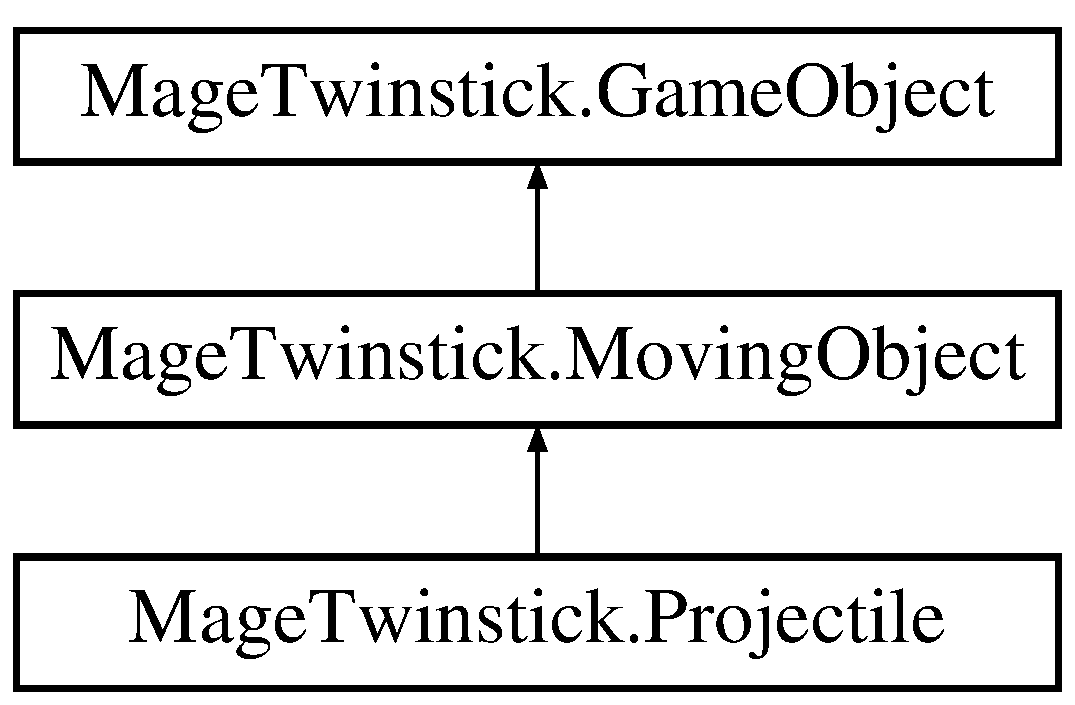
\includegraphics[height=4.000000cm]{class_mage_twinstick_1_1_projectile}
\end{center}
\end{figure}
\subsection*{Public Member Functions}
\begin{DoxyCompactItemize}
\item 
\hypertarget{class_mage_twinstick_1_1_projectile_a2e18fb2d662c973c867069a248b5a5ed}{}{\bfseries Projectile} (float speed, string image\+Path, \hyperlink{class_mage_twinstick_1_1_vector2_d}{Vector2\+D} start\+Pos, Rectangle display, float animation\+Speed)\label{class_mage_twinstick_1_1_projectile_a2e18fb2d662c973c867069a248b5a5ed}

\item 
\hypertarget{class_mage_twinstick_1_1_projectile_a9208eff25bc92289191d5470bbc7015a}{}override void {\bfseries Update} (float fps)\label{class_mage_twinstick_1_1_projectile_a9208eff25bc92289191d5470bbc7015a}

\item 
\hypertarget{class_mage_twinstick_1_1_projectile_ad646d013997eceb12a0ac2f5df56d3bb}{}override void {\bfseries On\+Collision} (\hyperlink{class_mage_twinstick_1_1_game_object}{Game\+Object} other)\label{class_mage_twinstick_1_1_projectile_ad646d013997eceb12a0ac2f5df56d3bb}

\end{DoxyCompactItemize}
\subsection*{Additional Inherited Members}


The documentation for this class was generated from the following file\+:\begin{DoxyCompactItemize}
\item 
Projectile.\+cs\end{DoxyCompactItemize}

\hypertarget{class_mage_twinstick_1_1_ranged_enemy}{}\section{Mage\+Twinstick.\+Ranged\+Enemy Class Reference}
\label{class_mage_twinstick_1_1_ranged_enemy}\index{Mage\+Twinstick.\+Ranged\+Enemy@{Mage\+Twinstick.\+Ranged\+Enemy}}


Inherits Mage\+Twinstick.\+Enemy.

\subsection*{Public Member Functions}
\begin{DoxyCompactItemize}
\item 
\hypertarget{class_mage_twinstick_1_1_ranged_enemy_ac9144b929ee221ab7ed7e0e497edfef8}{}{\bfseries Ranged\+Enemy} (float speed, int health, string image\+Path, \hyperlink{class_mage_twinstick_1_1_vector2_d}{Vector2\+D} start\+Pos, Rectangle display, float animation\+Speed)\label{class_mage_twinstick_1_1_ranged_enemy_ac9144b929ee221ab7ed7e0e497edfef8}

\end{DoxyCompactItemize}


The documentation for this class was generated from the following file\+:\begin{DoxyCompactItemize}
\item 
Ranged\+Enemy.\+cs\end{DoxyCompactItemize}

\hypertarget{class_mage_twinstick_1_1_unit}{}\section{Mage\+Twinstick.\+Unit Class Reference}
\label{class_mage_twinstick_1_1_unit}\index{Mage\+Twinstick.\+Unit@{Mage\+Twinstick.\+Unit}}
Inheritance diagram for Mage\+Twinstick.\+Unit\+:\begin{figure}[H]
\begin{center}
\leavevmode
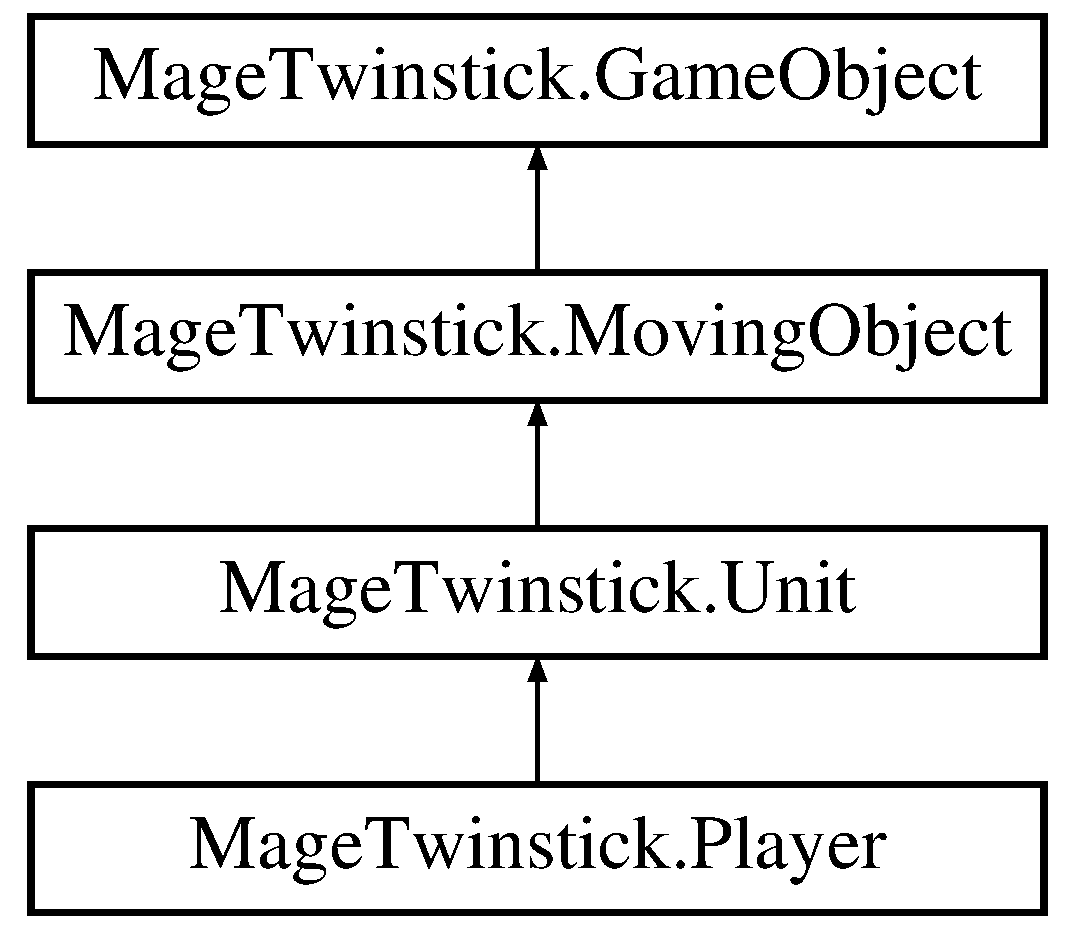
\includegraphics[height=4.000000cm]{class_mage_twinstick_1_1_unit}
\end{center}
\end{figure}
\subsection*{Public Member Functions}
\begin{DoxyCompactItemize}
\item 
\hyperlink{class_mage_twinstick_1_1_unit_a857d0f6e0f55b4c81e2a3bbf8711dd18}{Unit} (float speed, int health, string image\+Path, \hyperlink{class_mage_twinstick_1_1_vector2_d}{Vector2\+D} start\+Pos, Rectangle \hyperlink{class_mage_twinstick_1_1_game_object_a5807df7f837dc87c8955a008d0b27b50}{display}, float \hyperlink{class_mage_twinstick_1_1_game_object_a5d21c31402c27c5a19f2a62d98720456}{animation\+Speed})
\begin{DoxyCompactList}\small\item\em \hyperlink{class_mage_twinstick_1_1_unit}{Unit} Constructor \end{DoxyCompactList}\item 
abstract void \hyperlink{class_mage_twinstick_1_1_unit_a98b69920e6c6c09c5cfaacbf42a31bbf}{Attack} ()
\begin{DoxyCompactList}\small\item\em Abstract function Attack \end{DoxyCompactList}\end{DoxyCompactItemize}
\subsection*{Properties}
\begin{DoxyCompactItemize}
\item 
\hypertarget{class_mage_twinstick_1_1_unit_a5c06094e798c41a5d484f6ee00757667}{}double {\bfseries Health}\hspace{0.3cm}{\ttfamily  \mbox{[}get, set\mbox{]}}\label{class_mage_twinstick_1_1_unit_a5c06094e798c41a5d484f6ee00757667}

\end{DoxyCompactItemize}
\subsection*{Additional Inherited Members}


\subsection{Constructor \& Destructor Documentation}
\hypertarget{class_mage_twinstick_1_1_unit_a857d0f6e0f55b4c81e2a3bbf8711dd18}{}\index{Mage\+Twinstick\+::\+Unit@{Mage\+Twinstick\+::\+Unit}!Unit@{Unit}}
\index{Unit@{Unit}!Mage\+Twinstick\+::\+Unit@{Mage\+Twinstick\+::\+Unit}}
\subsubsection[{Unit(float speed, int health, string image\+Path, Vector2\+D start\+Pos, Rectangle display, float animation\+Speed)}]{\setlength{\rightskip}{0pt plus 5cm}Mage\+Twinstick.\+Unit.\+Unit (
\begin{DoxyParamCaption}
\item[{float}]{speed, }
\item[{int}]{health, }
\item[{string}]{image\+Path, }
\item[{{\bf Vector2\+D}}]{start\+Pos, }
\item[{Rectangle}]{display, }
\item[{float}]{animation\+Speed}
\end{DoxyParamCaption}
)\hspace{0.3cm}{\ttfamily [inline]}}\label{class_mage_twinstick_1_1_unit_a857d0f6e0f55b4c81e2a3bbf8711dd18}


\hyperlink{class_mage_twinstick_1_1_unit}{Unit} Constructor 


\begin{DoxyParams}{Parameters}
{\em speed} & \\
\hline
{\em health} & \\
\hline
{\em image\+Path} & \\
\hline
{\em start\+Pos} & \\
\hline
{\em display} & \\
\hline
{\em animation\+Speed} & \\
\hline
\end{DoxyParams}


\subsection{Member Function Documentation}
\hypertarget{class_mage_twinstick_1_1_unit_a98b69920e6c6c09c5cfaacbf42a31bbf}{}\index{Mage\+Twinstick\+::\+Unit@{Mage\+Twinstick\+::\+Unit}!Attack@{Attack}}
\index{Attack@{Attack}!Mage\+Twinstick\+::\+Unit@{Mage\+Twinstick\+::\+Unit}}
\subsubsection[{Attack()}]{\setlength{\rightskip}{0pt plus 5cm}abstract void Mage\+Twinstick.\+Unit.\+Attack (
\begin{DoxyParamCaption}
{}
\end{DoxyParamCaption}
)\hspace{0.3cm}{\ttfamily [pure virtual]}}\label{class_mage_twinstick_1_1_unit_a98b69920e6c6c09c5cfaacbf42a31bbf}


Abstract function Attack 



Implemented in \hyperlink{class_mage_twinstick_1_1_player_a418c80bddb416cd2cdd180ab21831f57}{Mage\+Twinstick.\+Player}.



The documentation for this class was generated from the following file\+:\begin{DoxyCompactItemize}
\item 
Unit.\+cs\end{DoxyCompactItemize}

\hypertarget{class_mage_twinstick_1_1_vector2_d}{}\section{Mage\+Twinstick.\+Vector2\+D Class Reference}
\label{class_mage_twinstick_1_1_vector2_d}\index{Mage\+Twinstick.\+Vector2\+D@{Mage\+Twinstick.\+Vector2\+D}}
\subsection*{Public Member Functions}
\begin{DoxyCompactItemize}
\item 
\hypertarget{class_mage_twinstick_1_1_vector2_d_a36be1b509d98d7ff48b7fff196a5bf23}{}{\bfseries Vector2\+D} (float x, float y)\label{class_mage_twinstick_1_1_vector2_d_a36be1b509d98d7ff48b7fff196a5bf23}

\item 
\hypertarget{class_mage_twinstick_1_1_vector2_d_a0675eb9cec3cd171d73797698e54f3ba}{}\hyperlink{class_mage_twinstick_1_1_vector2_d}{Vector2\+D} {\bfseries Subtract} (\hyperlink{class_mage_twinstick_1_1_vector2_d}{Vector2\+D} vec)\label{class_mage_twinstick_1_1_vector2_d_a0675eb9cec3cd171d73797698e54f3ba}

\item 
\hypertarget{class_mage_twinstick_1_1_vector2_d_a5b24373bc619c7fc5709bba32ca5303c}{}void {\bfseries Normalize} ()\label{class_mage_twinstick_1_1_vector2_d_a5b24373bc619c7fc5709bba32ca5303c}

\end{DoxyCompactItemize}
\subsection*{Properties}
\begin{DoxyCompactItemize}
\item 
float \hyperlink{class_mage_twinstick_1_1_vector2_d_ac750d49285ebcd4e4bb81295f91ab600}{X}\hspace{0.3cm}{\ttfamily  \mbox{[}get, set\mbox{]}}
\begin{DoxyCompactList}\small\item\em autoproperty for the X value \end{DoxyCompactList}\item 
float \hyperlink{class_mage_twinstick_1_1_vector2_d_a0ae54e599156e7c295515bfc80834bfd}{Y}\hspace{0.3cm}{\ttfamily  \mbox{[}get, set\mbox{]}}
\begin{DoxyCompactList}\small\item\em autoproperty for the Y value \end{DoxyCompactList}\end{DoxyCompactItemize}


\subsection{Property Documentation}
\hypertarget{class_mage_twinstick_1_1_vector2_d_ac750d49285ebcd4e4bb81295f91ab600}{}\index{Mage\+Twinstick\+::\+Vector2\+D@{Mage\+Twinstick\+::\+Vector2\+D}!X@{X}}
\index{X@{X}!Mage\+Twinstick\+::\+Vector2\+D@{Mage\+Twinstick\+::\+Vector2\+D}}
\subsubsection[{X}]{\setlength{\rightskip}{0pt plus 5cm}float Mage\+Twinstick.\+Vector2\+D.\+X\hspace{0.3cm}{\ttfamily [get]}, {\ttfamily [set]}}\label{class_mage_twinstick_1_1_vector2_d_ac750d49285ebcd4e4bb81295f91ab600}


autoproperty for the X value 

\hypertarget{class_mage_twinstick_1_1_vector2_d_a0ae54e599156e7c295515bfc80834bfd}{}\index{Mage\+Twinstick\+::\+Vector2\+D@{Mage\+Twinstick\+::\+Vector2\+D}!Y@{Y}}
\index{Y@{Y}!Mage\+Twinstick\+::\+Vector2\+D@{Mage\+Twinstick\+::\+Vector2\+D}}
\subsubsection[{Y}]{\setlength{\rightskip}{0pt plus 5cm}float Mage\+Twinstick.\+Vector2\+D.\+Y\hspace{0.3cm}{\ttfamily [get]}, {\ttfamily [set]}}\label{class_mage_twinstick_1_1_vector2_d_a0ae54e599156e7c295515bfc80834bfd}


autoproperty for the Y value 



The documentation for this class was generated from the following file\+:\begin{DoxyCompactItemize}
\item 
Vector2\+D.\+cs\end{DoxyCompactItemize}

%--- End generated contents ---

% Index
\backmatter
\newpage
\phantomsection
\clearemptydoublepage
\addcontentsline{toc}{chapter}{Index}
\printindex

\end{document}
